\documentclass[11pt,letterpaper]{article}
\usepackage[margin=1in]{geometry}
\usepackage[utf8]{inputenc}
\usepackage[T1]{fontenc}
\usepackage{microtype}
\usepackage{tgpagella}
\usepackage{booktabs}
\usepackage{tabularx}
\usepackage{array}
\usepackage{graphicx}
\usepackage[labelfont=bf,font=small,skip=6pt]{caption}
\usepackage{xcolor}
\usepackage{enumitem}
\definecolor{citationBlue}{HTML}{004B87}
\usepackage{hyperref}
\hypersetup{colorlinks=true, linkcolor=citationBlue, citecolor=citationBlue, urlcolor=citationBlue, pdfborder={0 0 0},
  pdftitle={BusyBox sort in biocontainers: Galaxy jobs that succeed with missing data}, pdfauthor={Richard Burhans}}
\setlist{itemsep=2pt, topsep=4pt}
\newcommand{\code}[1]{\texttt{#1}}
\newcommand{\VGP}[1]{\textcolor{orange}{[#1]}}

\title{\textbf{BusyBox \code{sort} in biocontainers:\\Galaxy jobs that succeed with missing data}}
\author{Richard Burhans\\\small Penn State University \quad ORCID \href{https://orcid.org/0009-0006-5949-0958}{0009-0006-5949-0958}}
\date{Technical note, 28 October 2026}

\begin{document}
\maketitle

\begin{abstract}
\noindent Most single-package biocontainers supply \code{sort} from BusyBox, which holds its entire input in
memory and silently ignores the options that make GNU \code{sort} spill to disk. When a job's memory limit kills
such a \code{sort} in the middle of a shell pipeline, the next command receives an empty or truncated stream, and
the pipeline still exits zero. Galaxy adds \code{set -e} to tool scripts but not \code{pipefail}, so the kill does
not reach the job's exit status. We reproduced this on usegalaxy.org and two other Galaxy servers. When Slurm's
memory limit killed \code{sort}, the job finished green with none of its 16.4 million lines in the output, even
though Slurm reported the kill on the job's standard error. Neither Pulsar, which ran those jobs, nor Galaxy's own
Slurm runner recognises that message.
We measure BusyBox \code{sort}'s memory use, which depends on line length in a way no simple multiple of the input
captures, and give five mitigations. The simplest is to sort to a file as a command of its own.
\end{abstract}

\section{The problem}

A Galaxy tool's command is a shell script run inside the tool's container. Biocontainers built from a single Bioconda
package start from a minimal base image whose basic utilities, \code{sort} among them, are the BusyBox multi-call
binary. In \code{quay.io/biocontainers/ucsc-maftobigmaf:482--h0b57e2e\_0}, \code{/usr/bin/sort} is BusyBox 1.36.1
(812{,}456 bytes, 380 hard links), and so is the \code{sort} of all 23 \code{ucsc-*} version 482 images we checked
(identical binary) and of the \code{blast}, \code{samtools} and \code{sourmash} images. Images whose packages pull
in \code{coreutils}, such as \code{multiz} and \code{kegalign-full}, have GNU \code{sort} first on the path instead.

BusyBox \code{sort} has no external merge. It reads every line into memory, sorts, and only then writes
(\code{coreutils/sort.c}). It accepts GNU's \code{-S} (buffer size) and \code{-T} (temporary directory) and
ignores them: sorting 1{,}000{,}000 lines peaked at 83.4\,MB without them and 83.8\,MB with \code{-S 1M -T
/tmp/spill}, and no file was written to the temporary directory. The long forms (\code{-{}-buffer-size},
\code{-{}-temporary-directory}, \code{-{}-parallel}) are rejected with exit status 2. A tool author who adds
\code{-S} and \code{-T} to stay within a memory limit gets no error and no protection. In BusyBox 1.32.1 the same
short options were rejected instead, which produced empty output files in Bismark~\cite{bismark483}.

\section{How much memory}

Peak memory grows with the number of lines as well as their bytes (Figure~\ref{fig:memory}). We sorted 50\,MB of
fixed-width numeric lines at 25 line lengths and read the peak from the container's control group. Lines of up to
112 bytes cost their own length plus 24 to 40 bytes. Lines of 120 to 256 bytes all cost about 275 bytes each,
whatever their length, so 120-byte lines need 2.5 times the input. Short lines are worst in ratio: 8-byte lines
needed 6.1 times the input. BusyBox reads each line into a buffer that grows in 256-byte steps and is then trimmed
(\code{libbb/get\_line\_from\_file.c}), which likely explains the step, but we did not trace the allocator.

\begin{figure}[ht]
\centering
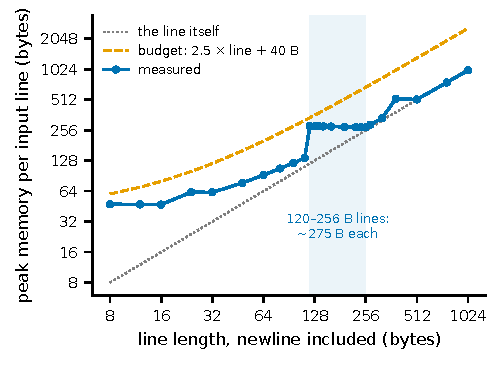
\includegraphics[width=0.62\textwidth]{figure1.pdf}
\caption{\textbf{BusyBox \code{sort}'s memory per line is not a fixed multiple of the line.} Peak memory per input
line (control-group peak minus an empty container's 5.9\,MB, divided by the line count) for 50\,MB of input at each
line length. Blue: measured. Grey dotted: the line itself. Orange dashed: the budget $2.5 \times$ line $+ 40$ bytes,
which covers every length measured. Shaded: lines of 120 to 256 bytes, which cost about 275 bytes each.}
\label{fig:memory}
\end{figure}

A budget that covers all 25 lengths is $6\,\mathrm{MB} + 2.5 \times \mathrm{input} + 40\,\mathrm{bytes} \times
\mathrm{lines}$. A rule stated as a multiple of the input alone undersizes short-line data such as identifier lists
or three-column BED by half or more.

\section{How the kill disappears}

A shell pipeline's exit status is that of its last command. When \code{sort} is killed mid-pipe, the consumer after
it sees end of input and exits normally. Table~\ref{tab:outcomes} shows what reached the consumer.

\begin{table}[ht]
\centering
\small
\caption{\textbf{A killed \code{sort} leaves the pipeline's exit status at zero.} Each row is
\code{\ldots{} | sort | awk 'END\{print NR\}'}. Docker rows: \code{docker -{}-memory} with swap disabled.}
\label{tab:outcomes}
\begin{tabularx}{\textwidth}{@{}>{\raggedright\arraybackslash}X l r r@{}}
\toprule
Setting & What killed \code{sort} & Exit status & Lines reaching the consumer \\
\midrule
Docker, 64\,MB, 2\,M lines from a file & its own growth while reading & 0 & 0 of 2{,}000{,}000 \\
Docker, same, with \code{pipefail} & its own growth while reading & 137 & 0 of 2{,}000{,}000 \\
Docker, 200\,MB, 60\,MB allocated by another process once output began & another process's growth & 0 & 401{,}222 of 2{,}000{,}000 \\
Galaxy (laila, Singularity), SIGKILL once output began & a signal & 0, job green & 242{,}248 of 2{,}000{,}000 \\
usegalaxy.org and vgp (Pulsar to Slurm, 512\,MiB), input from a file & its own growth while reading & 0, job green & 0 of 16{,}434{,}823 \\
usegalaxy.org and vgp (Pulsar to Slurm, 512\,MiB), live producer & its own growth while reading & 0, job green & 0 of 16{,}434{,}823 \\
usegalaxy.org and vgp (Pulsar to Slurm), SIGKILL once output began & a signal & 0, job green & 235{,}008 and 262{,}656 of 2{,}000{,}000 \\
\bottomrule
\end{tabularx}
\end{table}

If \code{sort} is killed while it reads, nothing has been written and the output is empty. If it is killed while it
writes, because some other process in the job grows, the output is cut at an arbitrary line. Either way, without
\code{pipefail}, the shell reports success. Which process the kernel kills is its own choice: with a live producer
in the same pipe, Docker's out-of-memory handling ended the whole container in every trial, which is loud.

The Galaxy rows are the result that matters. All three servers run Galaxy 26.1. On laila, a local server running
the job in Singularity, the job finished in state \code{ok} with exit code 0 and empty standard error, and its output
held 242{,}248 of 2{,}000{,}000 lines. On usegalaxy.org and vgp.usegalaxy.org, user-defined tools run through Pulsar
(\code{PulsarMQJobRunner}) on Jetstream2, which submits them to Slurm. There the job was given 512\,MiB and asked to sort 16{,}434{,}823 lines. Slurm enforced the limit (peak 536.8\,MB, one
out-of-memory kill in the job's control group), \code{sort} died while reading, and the consumer received nothing.
Every one of these jobs finished in state \code{ok} with exit code 0, and its output dataset held the single line
``0''. Slurm did notice: each job's standard error reads \code{slurmstepd: error: Detected 1 oom-kill event(s) in
StepId=\ldots. Some of your processes may have been killed by the cgroup out-of-memory handler.} Neither Pulsar
nor Galaxy acted on it.

\section{Why Galaxy does not catch it}

Galaxy prefixes a tool's script with \code{set -e} when the tool is strict, which is the default for XML tools with
\code{profile} 20.09 or later and always the case for YAML and user-defined tools. It never adds \code{pipefail}.
Under \code{set -e} a pipeline fails only if its last command fails. A proposal to add \code{pipefail} to every tool
script was discussed in 2018 to 2020 and closed, partly because \code{pipefail} ``is not POSIX so it may not work
when executing jobs on containers (which use \code{sh} instead of \code{bash})''~\cite{galaxy5884}. Galaxy does run
containerised scripts as \code{/bin/sh}, but in every biocontainer we checked, \code{/bin/sh} is bash.
\code{detect\_errors="exit\_code"} sees only the exit status, and a SIGKILL writes nothing to standard error, so
\code{detect\_errors="aggressive"} would not catch it either.

The jobs above ran through Pulsar, which does not read Slurm's memory messages at all, a known gap~\cite{galaxy24545}.
Galaxy's own Slurm runner, used where Galaxy submits to Slurm directly, has out-of-memory detection, but by its
source it would miss this case too, for two reasons
(\code{lib/galaxy/jobs/runners/slurm.py}, lines 29--42 and 210--226). It looks for Slurm's older wording,
\code{Exceeded job memory limit}, not the \code{Detected N oom-kill event(s)} that current Slurm writes. It fails a job
outright when Slurm reports the state \code{OUT\_OF\_MEMORY}, and reads the job's standard error for a memory
message only when Slurm reports the job as cancelled, and a job whose script exited 0 is reported as completed. The message also lands in the job's standard error rather than the tool's, so a tool's own
standard-error checks would probably not see it (we did not test this).

\section{Mitigations}

\begin{enumerate}
\item \textbf{Sort to a file, as a command of its own.} \code{sort -k1,1 -k2,2n -o sorted.bed in.bed}. A kill then
sets the exit status of a top-level command, which \code{set -e} sees. This needs no \code{pipefail} and has no false
failures.
\item \textbf{If the sort must stay in a pipe, set \code{pipefail} inside the script that runs it.} A child shell
does not inherit it, so a tool that runs a configuration-file script needs it in that script. Do not follow the sort
with a consumer that stops early: under \code{pipefail}, \code{sort | head -1} exits 141 when \code{head} closes
the pipe, the failure Galaxy's own ``Show beginning'' tool hit in 2021~\cite{galaxy12093}.
\item \textbf{Use GNU \code{sort} for large inputs} by adding a \code{coreutils} requirement, so that the tool runs in
a multi-package container with GNU \code{sort} first on the path~\cite{iuc3920}. GNU \code{sort} spills to disk:
in one trial it finished 2{,}000{,}000 lines under a 64\,MB limit. User-defined tools resolve no requirements, so
for them only the container itself decides.
\item \textbf{Lint for it.} A rule that flags \code{sort} anywhere but last in a pipeline, unless the tool requires
\code{coreutils}, would reach every tool author through \code{planemo lint}. We wrote a prototype that parses each
tool with Galaxy's own parser. On the 2{,}061 tools in \code{galaxyproject/tools-iuc} (commit \code{ba9ee7d1}) it
flags 6, 5 of them without a \code{coreutils} requirement. Only one sorts input whose size grows with the data: the
Ensembl VEP wrapper's sort of a user-supplied annotation file, and that wrapper sets \code{pipefail}, so a kill
would fail the job. The other four sort short lists. The collection is not exposed today, so the rule's value is in
catching the next wrapper. (Its review shows the convention that makes this matter: ``sort is coreutils and I
thought we do not normally require that''~\cite{iuc4533}.)
\item \textbf{Have the job runners recognise the kill.} Treating \code{Detected N oom-kill event(s)} in a job's
standard error as a memory failure, whatever the exit status, in Pulsar and in Galaxy's Slurm runner, would have
failed every Slurm job in Table~\ref{tab:outcomes} except the SIGKILL control. A cleaner option, suggested in the
Galaxy discussion~\cite{galaxy24545}, is a destination setting that reads the job's control-group
\code{memory.events} directly. Either fixes every tool at once.
\end{enumerate}

\noindent Where none of these applies, size the job with the budget above, and check that a sort's output has as
many lines as its input wherever that count cannot change (not with \code{sort -u}).

\section{Prior reports}

BusyBox \code{sort}'s in-memory design is known: an nf-core module failed on large inputs for that reason in
2026~\cite{nfcore13033}, loudly, because the calling program checked the result. A coreutils requirement was added
to the tools-iuc \code{vcfsort} wrapper because BusyBox \code{sort} lacks \code{-V}~\cite{iuc3920}. We found no
report of a mid-pipe kill producing a successful job with missing data, and none of \code{-S} and \code{-T} being
silently ignored (GitHub issue search, 28 October 2026, queries listed in the repository).

\section*{Methods and availability}

All measurements, scripts and raw outputs are at
\href{https://github.com/richard-burhans/technical-notes}{github.com/richard-burhans/technical-notes} under
\code{busybox-sort/}. Container measurements: \code{probe/probe\_container.py}, Docker with cgroup v2, image
\code{quay.io/biocontainers/ucsc-maftobigmaf:482--h0b57e2e\_0}. Galaxy measurements: \code{probe/probe\_galaxy.py},
which registers a user-defined tool (\code{probe/busybox\_sort\_probe.gxtool.yml}) and records each job's state,
exit code, streams, metrics and output (\code{measurements/galaxy\_runs.jsonl}). Galaxy runs: laila with tool
version 0.1.0, usegalaxy.org and vgp.usegalaxy.org with version 0.2.0, all Galaxy 26.1.2.dev0, 28 October 2026. Galaxy
source citations are to \code{galaxyproject/galaxy} at \code{3d263f95ed} (\code{lib/galaxy/jobs/command\_factory.py},
lines 210--216). Lint prototype: \code{probe/check\_midpipe\_sort.py}. This note, its figure and its code are
dedicated to the public domain under CC0 1.0.

\begin{thebibliography}{9}
\small
\bibitem{bismark483} BioContainers/containers issue 483, ``bismark container Linux sort version'' (2022).
\url{https://github.com/BioContainers/containers/issues/483}
\bibitem{galaxy5884} galaxyproject/galaxy issue 5884, ``pipefail and errexit in all tool\_scripts'' (2018--2022).
\url{https://github.com/galaxyproject/galaxy/issues/5884}
\bibitem{galaxy12093} galaxyproject/galaxy issue 12093, ``Show beginning1 fails on any file longer than the number of
lines requested'' (2021), fixed in pull request 12112. \url{https://github.com/galaxyproject/galaxy/issues/12093}
\bibitem{galaxy24545} galaxyproject/galaxy issue 24545, ``Slurm runner: an OOM-killed process can leave the job
\code{ok}'' (2026), with the maintainers' replies. \url{https://github.com/galaxyproject/galaxy/issues/24545}
\bibitem{iuc3920} galaxyproject/tools-iuc pull request 3920, ``Add coreutils requirement to vcfsort'' (2021).
\url{https://github.com/galaxyproject/tools-iuc/pull/3920}
\bibitem{iuc4533} galaxyproject/tools-iuc pull request 4533, ``Add Ensembl VEP (Variant Effect Predictor) tool and
corresponding data manager'' (2022), review of \code{ensembl\_vep.xml}. \url{https://github.com/galaxyproject/tools-iuc/pull/4533}
\bibitem{nfcore13033} nf-core/modules issue 13033, ``hmmer/eslsfetchindex: fails on large FASTA in containers (BusyBox
sort in biocontainers image)'' (2026). \url{https://github.com/nf-core/modules/issues/13033}
\end{thebibliography}

\end{document}
